% Hook lengths of (5,4,2,1) and one hook walk. Generated by a short script.
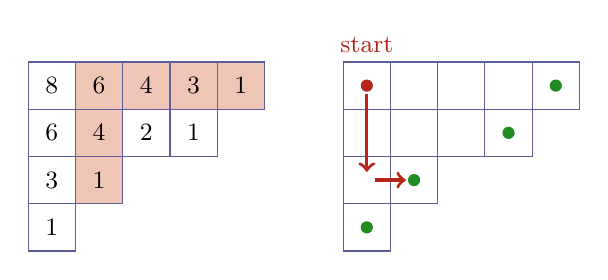
\begin{tikzpicture}[font=\small]
\fill[BrickRed!20] (0.60,0.00) rectangle (1.20,-0.60);
\fill[BrickRed!20] (1.20,0.00) rectangle (1.80,-0.60);
\fill[BrickRed!20] (1.80,0.00) rectangle (2.40,-0.60);
\fill[BrickRed!20] (2.40,0.00) rectangle (3.00,-0.60);
\fill[BrickRed!20] (0.60,-0.60) rectangle (1.20,-1.20);
\fill[BrickRed!20] (0.60,-1.20) rectangle (1.20,-1.80);
\draw[MidnightBlue!70] (0.00,0.00) rectangle (0.60,-0.60);
\node at (0.30,-0.30) {$8$};
\draw[MidnightBlue!70] (0.60,0.00) rectangle (1.20,-0.60);
\node at (0.90,-0.30) {$6$};
\draw[MidnightBlue!70] (1.20,0.00) rectangle (1.80,-0.60);
\node at (1.50,-0.30) {$4$};
\draw[MidnightBlue!70] (1.80,0.00) rectangle (2.40,-0.60);
\node at (2.10,-0.30) {$3$};
\draw[MidnightBlue!70] (2.40,0.00) rectangle (3.00,-0.60);
\node at (2.70,-0.30) {$1$};
\draw[MidnightBlue!70] (0.00,-0.60) rectangle (0.60,-1.20);
\node at (0.30,-0.90) {$6$};
\draw[MidnightBlue!70] (0.60,-0.60) rectangle (1.20,-1.20);
\node at (0.90,-0.90) {$4$};
\draw[MidnightBlue!70] (1.20,-0.60) rectangle (1.80,-1.20);
\node at (1.50,-0.90) {$2$};
\draw[MidnightBlue!70] (1.80,-0.60) rectangle (2.40,-1.20);
\node at (2.10,-0.90) {$1$};
\draw[MidnightBlue!70] (0.00,-1.20) rectangle (0.60,-1.80);
\node at (0.30,-1.50) {$3$};
\draw[MidnightBlue!70] (0.60,-1.20) rectangle (1.20,-1.80);
\node at (0.90,-1.50) {$1$};
\draw[MidnightBlue!70] (0.00,-1.80) rectangle (0.60,-2.40);
\node at (0.30,-2.10) {$1$};
\draw[MidnightBlue!70] (4.00,0.00) rectangle (4.60,-0.60);
\draw[MidnightBlue!70] (4.60,0.00) rectangle (5.20,-0.60);
\draw[MidnightBlue!70] (5.20,0.00) rectangle (5.80,-0.60);
\draw[MidnightBlue!70] (5.80,0.00) rectangle (6.40,-0.60);
\draw[MidnightBlue!70] (6.40,0.00) rectangle (7.00,-0.60);
\draw[MidnightBlue!70] (4.00,-0.60) rectangle (4.60,-1.20);
\draw[MidnightBlue!70] (4.60,-0.60) rectangle (5.20,-1.20);
\draw[MidnightBlue!70] (5.20,-0.60) rectangle (5.80,-1.20);
\draw[MidnightBlue!70] (5.80,-0.60) rectangle (6.40,-1.20);
\draw[MidnightBlue!70] (4.00,-1.20) rectangle (4.60,-1.80);
\draw[MidnightBlue!70] (4.60,-1.20) rectangle (5.20,-1.80);
\draw[MidnightBlue!70] (4.00,-1.80) rectangle (4.60,-2.40);
\fill[ForestGreen] (6.70,-0.30) circle (2.2pt);
\fill[ForestGreen] (6.10,-0.90) circle (2.2pt);
\fill[ForestGreen] (4.90,-1.50) circle (2.2pt);
\fill[ForestGreen] (4.30,-2.10) circle (2.2pt);
\fill[BrickRed] (4.30,-0.30) circle (2.2pt);
\draw[BrickRed,very thick,->,shorten >=3pt,shorten <=3pt] (4.30,-0.30) -- (4.30,-1.50);
\draw[BrickRed,very thick,->,shorten >=3pt,shorten <=3pt] (4.30,-1.50) -- (4.90,-1.50);
\node[BrickRed,above] at (4.30,0.0) {start};
\end{tikzpicture}
